\documentclass[11pt,twocolumn]{article}

\usepackage[utf8]{inputenc}
\usepackage[T1]{fontenc}
\usepackage{lmodern}
\usepackage[margin=1in]{geometry}
\usepackage{amsmath,amssymb}
\usepackage{booktabs}
\usepackage{tabularx}
\usepackage{multirow}
\usepackage{graphicx}
\usepackage{xcolor}
\usepackage{hyperref}
\usepackage{cleveref}
\usepackage{pgfplots}
\usepackage{pgfplotstable}
\pgfplotsset{compat=1.18}
\usepackage{enumitem}
\usepackage{microtype}
\usepackage{float}
\usepackage{subcaption}
\usepackage{siunitx}

\sisetup{group-separator={,}}

\definecolor{positive}{RGB}{0,128,0}
\definecolor{negative}{RGB}{192,0,0}

\newcommand{\improve}[1]{\textcolor{positive}{\textbf{#1}}}
\newcommand{\regress}[1]{\textcolor{negative}{\textbf{#1}}}

\title{Optimizing Hash Array Mapped Tries in Go:\\
Allocation Strategies, Fanout Tuning, and Cache Effects}

\author{%
  Marcelo Cantos\textsuperscript{1} \and
  Claude\textsuperscript{2} \\[6pt]
  \textsuperscript{1}arr.ai \\
  \textsuperscript{2}Anthropic
}

\date{February 2026}

\begin{document}

\maketitle

% ============================================================================
\begin{abstract}
Hash array mapped tries (HAMTs) are a foundational data structure for
persistent collections in functional and immutable programming.
We present an empirical study of HAMT optimization in Go, motivated by
performance regressions introduced during a node-type simplification of the
\texttt{frozen} immutable collections library.
Through CPU and memory profiling, we identified three optimization techniques
--- boxing elimination via per-type function caching, hot-path bypass of
concurrent map lookups, and inline structural copying --- that collectively
reduced merge-path allocations by 75\% and improved merge throughput by 38\%.
We further conducted a systematic exploration of branching factor (4, 8, 16, 32),
including empirical measurement of branch occupancy and cache-line utilization
on both x86-64 and Apple Silicon architectures.
Our occupancy analysis reveals that 8-way branching achieves 95\% slot
utilization, explaining why neither wider nor narrower fanouts improve overall
performance: wider nodes waste copy bandwidth on empty slots, while narrower
nodes increase tree depth and allocation count.
We conclude that in garbage-collected languages with interface-based
polymorphism, \emph{allocation count} dominates \emph{allocation size} as the
primary performance lever, and that branching factor selection must account for
language-specific overhead per node rather than asymptotic depth alone.
\end{abstract}

% ============================================================================
\section{Introduction}
\label{sec:introduction}

Immutable data structures provide referential transparency, safe concurrent
access without locking, and straightforward undo/versioning semantics.
Among them, the hash array mapped trie (HAMT), introduced by
Bagwell~\cite{bagwell2001}, has become the standard backing structure for
persistent hash maps and sets in languages such as
Clojure~\cite{hickey2008}, Scala~\cite{odersky2004}, and
Haskell~\cite{tibell2014}.

HAMTs achieve near-$O(1)$ amortized access by partitioning hash bits into
fixed-width chunks that index into trie levels, with structural sharing
ensuring that mutations allocate only $O(\log n)$ new nodes.
However, the constant factors hidden in this complexity are
language-dependent: pointer size, GC pressure, cache behavior, and dispatch
overhead all vary significantly across runtimes.

Go presents a distinctive set of constraints for HAMT implementation.
Its generics (introduced in Go~1.18~\cite{go118}) use dictionary-based
dispatch rather than monomorphization, causing type-parameterized functions
to box values through empty interfaces.
Its garbage collector is a concurrent, tri-color mark-sweep collector
optimized for low pause times but sensitive to allocation
rate~\cite{hudson2018}.
And its escape analysis, while sophisticated, conservatively heap-allocates
values that are returned by pointer or stored in interfaces.

In this paper, we report on a systematic optimization campaign for
\texttt{frozen}\footnote{\url{https://github.com/arr-ai/frozen}}, a Go
library providing immutable \texttt{Set[T]}, \texttt{Map[K,V]}, and
\texttt{IntSet[I]} types backed by a HAMT.
A simplification that reduced four node types to two introduced regressions
of up to 56\% on merge-heavy benchmarks.
Through profiling-driven optimization and systematic exploration of
structural parameters, we:

\begin{enumerate}[nosep]
  \item Eliminated boxing allocations on equality and hash hot paths
        (\cref{sec:boxing}).
  \item Removed per-operation concurrent map lookups from the mutable
        builder (\cref{sec:syncmap}).
  \item Halved per-level allocations on immutable path-copy operations
        (\cref{sec:inline}).
  \item Conducted a controlled experiment across four branching factors
        (4, 8, 16, 32) with empirical occupancy and cache-line analysis
        (\cref{sec:fanout}).
  \item Evaluated compact (variable-length) node arrays against the
        measured occupancy profile (\cref{sec:compact}).
\end{enumerate}

% ============================================================================
\section{Background and Related Work}
\label{sec:related}

\subsection{Hash Array Mapped Tries}

Bagwell's original HAMT~\cite{bagwell2001} uses a bitmap and a compact
(popcount-indexed) child array at each node, with a configurable chunk size
$t$ (typically 5 bits, yielding a fanout of 32).
Immutable variants allocate new nodes along the root-to-leaf path on each
update (``path copying''), sharing all other subtrees with the previous
version~\cite{driscoll1989}.

\subsection{CHAMP and Lean Tries}

Steindorfer and Vinju~\cite{steindorfer2015} introduced the Compressed
Hash-Array Mapped Prefix-tree (CHAMP), which separates inline values from
sub-node pointers in the node layout, achieving 1.3--6.7$\times$ iteration
speedup on the JVM.
Their work demonstrated that node-level memory layout significantly impacts
performance, even when asymptotic complexity is unchanged.

\subsection{Branching Factor Studies}

The choice of branching factor $b = 2^t$ involves a tradeoff: larger $b$
reduces tree depth (and thus pointer chases per lookup) but increases node
size (and thus copy cost per mutation).
Stucki et al.~\cite{stucki2015} explored this for RRB-trees, finding that
$b = 32$ is optimal for JVM arrays.
Prokopec et al.~\cite{prokopec2012} analyzed concurrent tries with
$b = 32$ on the JVM.
However, these results assume compact (popcount-indexed) arrays and JVM
object headers; neither applies directly to Go.

\subsection{Go Runtime Characteristics}

Go's garbage collector performs concurrent mark-and-sweep with sub-millisecond
pause times~\cite{hudson2018}.
Its cost is proportional to the number of live pointers, making data
structures with many small pointer-containing objects (such as HAMT branches)
particularly GC-sensitive.
Go generics use runtime dictionaries for type-parameterized
functions~\cite{go118}, which can cause implicit heap allocation (``boxing'')
when values are passed through \texttt{interface\{\}} parameters.
These characteristics create a unique optimization landscape where reducing
allocation count per operation is often more impactful than reducing
allocation size.

% ============================================================================
\section{System Under Study}
\label{sec:system}

\subsection{Architecture}

The \texttt{frozen} HAMT uses $t = 3$ (fanout $b = 8$) by default, with
multi-round hashing: when all $\lfloor 64/3 \rfloor = 21$ levels of a
64-bit hash are exhausted, a new hash is generated with a different seed.
This eliminates the need for overflow buckets.

Node types after the triggering simplification:

\begin{description}[nosep,leftmargin=1em]
  \item[\texttt{branch[T]}] Internal node: 16-bit occupancy mask,
    \texttt{[8]node[T]} child array (8 Go interfaces = 128 bytes), element
    count. Total: 144 bytes.
  \item[\texttt{leaf1[T]}] Single-element leaf (16 bytes).
  \item[\texttt{leaf[T]}] Multi-element leaf (2--8 elements) with linear scan.
    Defers branch creation until a 9th element arrives.
\end{description}

The \texttt{node[T]} interface is a Go interface (16 bytes: type pointer +
data pointer), providing polymorphic dispatch at the cost of indirect calls
and GC tracing overhead per slot.

\subsection{Operations}

\begin{description}[nosep,leftmargin=1em]
  \item[\texttt{With}] Immutable insertion: path-copies from root to leaf,
    returning a new tree. Uses \texttt{WithFast} (no combine function) on
    the fast path.
  \item[\texttt{Builder.Add}] Mutable insertion: modifies nodes in place.
    Used for batch construction.
  \item[\texttt{Combine}] Merge of two trees (used for \texttt{Set.Union},
    \texttt{Map.Merge}). Traverses both trees, creating new branches where
    they overlap.
  \item[\texttt{Without}] Immutable removal: path-copies with potential
    node collapse.
\end{description}

\subsection{Experimental Setup}

All benchmarks were run on an Apple M4 Max (12 performance + 4 efficiency
cores, 128-byte L1 cache lines on performance cores) with Go~1.25.7.
Each benchmark used 5 iterations via \texttt{go test -bench -count=5} and
was compared using \texttt{benchstat}~\cite{benchstat} for statistical
significance.
We report time/op, bytes/op (B/op), and allocations/op (allocs/op).

% ============================================================================
\section{Optimization 1: Boxing Elimination}
\label{sec:boxing}

\subsection{Problem}

Go's generic functions receive type-parameterized values via runtime
dictionaries.
When a generic function calls a method through an interface conversion ---
e.g., \texttt{any(key).(hash.Hashable).Hash(seed)} --- the value \texttt{key}
is ``boxed'': copied to the heap and wrapped in an interface value.
In the HAMT hot paths, every element comparison and hash computation
triggered a boxing allocation.

\subsection{Solution}

We introduced a per-type function cache using \texttt{sync.Map}, keyed by
\texttt{reflect.TypeOf(\&t)} (using a pointer type to avoid the boxing that
\texttt{TypeOf(t)} would cause for value types):

\begin{verbatim}
func resolveHashFunc[T any]()
    func(T, uintptr) uintptr {
  var t T
  switch unsafe.Sizeof(t) {
  case 1: return func(k T, s uintptr)
      uintptr {
    return hash.Uint8(
      *(*uint8)(unsafe.Pointer(&k)), s)
  }
  // ... cases for 2, 4, 8 bytes
  }
  return func(k T, s uintptr) uintptr {
    return hash.Any(k, s) // fallback
  }
}
\end{verbatim}

The resolver runs once per type instantiation.
Subsequent calls retrieve the cached function via \texttt{sync.Map.Load},
which returns a non-boxing, type-specialized closure.
An equivalent resolver handles equality comparisons, with special cases for
floating-point types (which require NaN-aware comparison).

\subsection{Results}

\Cref{tab:boxing} shows the impact on key benchmarks.

\begin{table}[h]
\centering
\caption{Impact of boxing elimination (vs.\ pre-optimization baseline).}
\label{tab:boxing}
\begin{tabular}{@{}lrrr@{}}
\toprule
Benchmark & Time & B/op & Allocs \\
\midrule
SetBuilder 1Mi  & $-18\%$ & $-46\%$ & $-75\%$ \\
MergeFrozenMap 1M & $-25\%$ & $-42\%$ & $-80\%$ \\
SetParallelWith 1M & $-15\%$ & --- & --- \\
\bottomrule
\end{tabular}
\end{table}

The allocation reduction is dramatic because boxing was occurring on
\emph{every} comparison and hash computation --- $O(n \log n)$ times for
$n$-element operations.

% ============================================================================
\section{Optimization 2: \texttt{sync.Map} Bypass}
\label{sec:syncmap}

\subsection{Problem}

After boxing elimination, CPU profiling of \texttt{SetBuilder.Add} at
$n = 1024$ revealed that \texttt{sync.Map.Load} consumed 16.75\% of CPU
time.
Each \texttt{Add} performed two \texttt{sync.Map} lookups per element: one
for the hash function and one for the equality function.
While \texttt{sync.Map} is lock-free on the read path, it still involves
atomic loads and interface assertions that are significant on a hot loop.

\subsection{Solution}

We pre-resolve both functions at \texttt{Builder} construction time into a
\texttt{CombineArgs[T]} struct:

\begin{verbatim}
type Builder[T any] struct {
  t    Tree[T]
  args *CombineArgs[T]
}
\end{verbatim}

The \texttt{CombineArgs} are themselves cached per type in a
\texttt{sync.Map}, amortizing the one-time lookup across all
\texttt{Builder} instances of the same type.
A lazy initialization guard (\texttt{if b.args == nil}) handles the
zero-value \texttt{Builder} case, since Go allows
\texttt{var b Builder[T]} without calling a constructor.

\subsection{Results}

\begin{table}[h]
\centering
\caption{Impact of \texttt{sync.Map} bypass (cumulative with boxing fix).}
\label{tab:syncmap}
\begin{tabular}{@{}lrrr@{}}
\toprule
Benchmark & Time & B/op & Allocs \\
\midrule
SetBuilder 32   & $-17\%$ & $-23\%$ & $-24\%$ \\
SetBuilder 1ki  & $-35\%$ & $-23\%$ & $-45\%$ \\
SetUnion 1M     & $-29\%$ & --- & --- \\
\bottomrule
\end{tabular}
\end{table}

An initial implementation caused a +157\% regression on \texttt{IntSet/New/100}
because \texttt{CombineArgs} was allocated per \texttt{Builder} instance (5
extra allocations, 96 bytes).
Caching the args per type in a \texttt{sync.Map} resolved this, restoring
\texttt{IntSet/New} to 1 allocation and 16 B/op.

% ============================================================================
\section{Optimization 3: Inline Branch Copies}
\label{sec:inline}

\subsection{Problem}

The immutable \texttt{WithFast} method performed two heap allocations per
branch level:

\begin{verbatim}
ret := newBranch(b.p.WithChild(i, x2))
\end{verbatim}

\texttt{packer.WithChild} allocates a copy of the packer struct (returned
as \texttt{*packer[T]}), then \texttt{newBranch} allocates a \texttt{branch}
and copies the packer into it.
For a tree of depth $d$, each \texttt{With} operation produced $2d$
allocations.

\subsection{Solution}

Copy the branch by value and return a pointer to the copy:

\begin{verbatim}
ret := *b               // struct copy
ret.p.data[i] = x2      // modify the copy
ret.count = b.count + 1 - matches
return &ret, matches
\end{verbatim}

Go's escape analysis detects that \texttt{ret} escapes via \texttt{\&ret}
and allocates it on the heap --- but as a single allocation.
This pattern was already used by the mutable \texttt{Remove} method; we
extended it to \texttt{with}, \texttt{WithFast}, and \texttt{Without}.
The unused \texttt{packer.updateMaskBit} method and the \texttt{masker}
import were removed as dead code.

\subsection{Results}

\begin{table}[h]
\centering
\caption{Impact of inline branch copies (cumulative with previous fixes).}
\label{tab:inline}
\begin{tabular}{@{}lrrr@{}}
\toprule
Benchmark & Time & B/op & Allocs \\
\midrule
SetBuilder 32   & $-17\%$ & --- & $-24\%$ \\
Set-With 32     & $-12\%$ & --- & $-9\%$ \\
Set-With 1ki    & $-5\%$ & --- & --- \\
IntSet/With 1M  & $-8\%$ & --- & --- \\
InsertFrozenMap 1k & $-10\%$ & --- & $-10\%$ \\
MergeFrozenMap 1M  & $-6\%$ & --- & --- \\
\bottomrule
\end{tabular}
\end{table}

% ============================================================================
\section{Cumulative Impact}
\label{sec:cumulative}

\Cref{tab:cumulative} presents the net effect of all three optimizations
against the pre-simplification baseline.

\begin{table}[h]
\centering
\caption{Cumulative impact of all optimizations vs.\ original baseline.
  Positive values (red) indicate regressions.}
\label{tab:cumulative}
\begin{tabular}{@{}lrrr@{}}
\toprule
Benchmark & Time & B/op & Allocs \\
\midrule
SetBuilder 32   & \improve{$-31\%$} & $-38\%$ & $-34\%$ \\
SetBuilder 1ki  & \improve{$-4.5\%$} & $-24\%$ & $-46\%$ \\
MergeFrozenMap 1M & \improve{$-38\%$} & $-62\%$ & $-75\%$ \\
SetUnion 1M     & \improve{$-46\%$} & $-37\%$ & --- \\
SetParallelWith 1M & \improve{$-17\%$} & --- & --- \\
\midrule
Set-With 32     & \regress{$+30\%$} & $-4\%$ & $-9\%$ \\
Set-With 1ki    & \regress{$+22\%$} & $-4\%$ & --- \\
Set-With 1Mi    & \regress{$+14\%$} & --- & --- \\
IntSet/With 100 & \regress{$+62\%$} & $+21\%$ & --- \\
\bottomrule
\end{tabular}
\end{table}

Merge and builder paths now significantly exceed the original baseline.
Set-With remains regressed due to structural changes in the simplified node
types.

\begin{figure}[h]
\centering
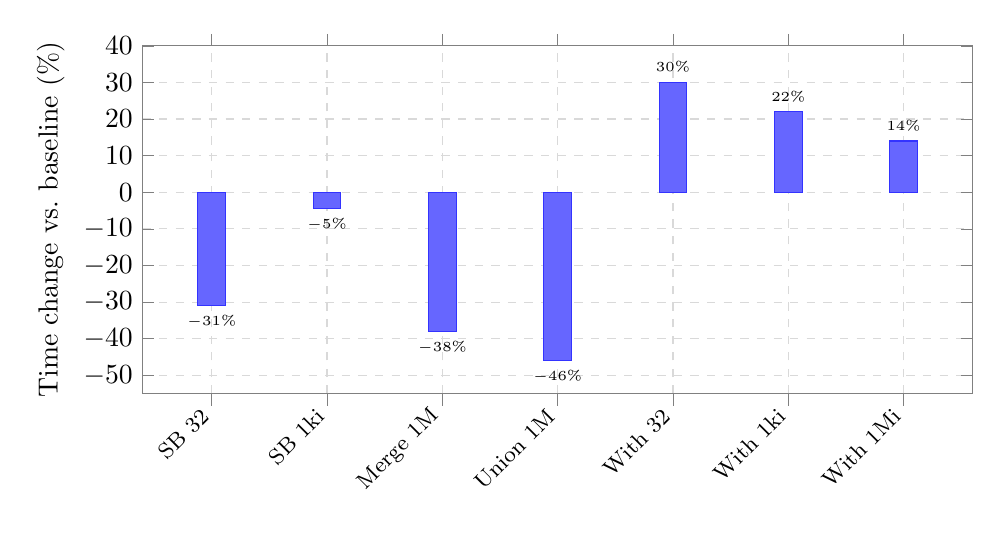
\begin{tikzpicture}
\begin{axis}[
    ybar,
    width=\columnwidth,
    height=6cm,
    ylabel={Time change vs.\ baseline (\%)},
    symbolic x coords={
      {SB 32},{SB 1ki},{Merge 1M},{Union 1M},{With 32},{With 1ki},{With 1Mi}
    },
    xtick=data,
    x tick label style={rotate=45, anchor=east, font=\footnotesize},
    ymin=-55, ymax=40,
    ytick={-50,-40,-30,-20,-10,0,10,20,30,40},
    bar width=10pt,
    nodes near coords={\pgfmathprintnumber\pgfplotspointmeta\%},
    nodes near coords style={font=\tiny, rotate=0},
    every node near coord/.append style={
      /pgfplots/point meta=explicit,
    },
    grid=major,
    grid style={dashed, gray!30},
    axis line style={gray},
]
\addplot[
    fill=blue!60,
    draw=blue!80,
    point meta=explicit,
] coordinates {
    ({SB 32}, -31) [-31]
    ({SB 1ki}, -4.5) [-5]
    ({Merge 1M}, -38) [-38]
    ({Union 1M}, -46) [-46]
    ({With 32}, 30) [30]
    ({With 1ki}, 22) [22]
    ({With 1Mi}, 14) [14]
};
\end{axis}
\end{tikzpicture}
\caption{Cumulative time change for key benchmarks after all three
  optimizations, relative to the pre-simplification baseline.
  Negative values indicate improvement.}
\label{fig:cumulative}
\end{figure}

% ============================================================================
\section{Fanout Exploration}
\label{sec:fanout}

\subsection{Motivation}

The remaining Set-With regression is dominated by allocation cost on the
immutable path-copy.
Each \texttt{With} allocates one branch per tree level.
Wider branching reduces depth (and thus allocations) but increases the size
of each branch copy.
We hypothesized that an alternative fanout might yield a better tradeoff.

\subsection{Branch Occupancy}
\label{sec:occupancy}

We instrumented the tree to measure the fraction of populated slots at each
depth for a tree of $n = 10^6$ elements.
\Cref{tab:occupancy} presents results for fanout 8 and fanout 32.

\begin{table}[h]
\centering
\caption{Branch occupancy by depth for $n = 10^6$ elements.}
\label{tab:occupancy}
\begin{tabular}{@{}lrrrr@{}}
\toprule
& \multicolumn{2}{c}{Fanout 8} & \multicolumn{2}{c}{Fanout 32} \\
\cmidrule(lr){2-3} \cmidrule(lr){4-5}
Depth & Branches & Occ. & Branches & Occ. \\
\midrule
0     & 1       & 100\% & 1       & 50\% \\
1     & 8       & 100\% & 32      & 50\% \\
2     & 64      & 100\% & 1,024   & 50\% \\
3     & 512     & 100\% & 32,768  & 31\% \\
4     & 4,096   & 100\% & ---     & --- \\
5     & 32,768  & 98\%  & ---     & --- \\
6     & 4,273   & 72\%  & ---     & --- \\
\midrule
\textbf{Total} & \textbf{41,722} & \textbf{95\%} & \textbf{33,825} & \textbf{31\%} \\
\bottomrule
\end{tabular}
\end{table}

\begin{figure}[h]
\centering
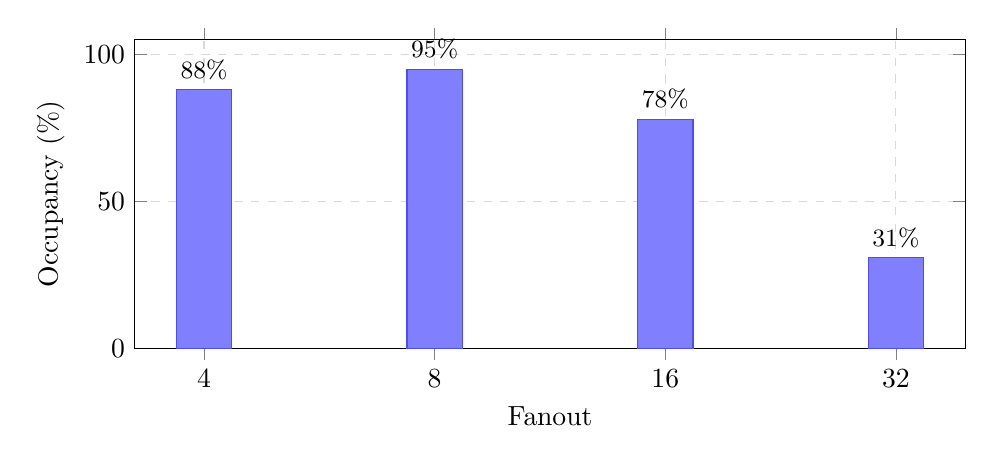
\begin{tikzpicture}
\begin{axis}[
    ybar,
    width=\columnwidth,
    height=5.5cm,
    ylabel={Occupancy (\%)},
    xlabel={Fanout},
    symbolic x coords={4, 8, 16, 32},
    xtick=data,
    ymin=0, ymax=105,
    bar width=20pt,
    nodes near coords={\pgfmathprintnumber\pgfplotspointmeta\%},
    nodes near coords style={font=\small},
    grid=major,
    grid style={dashed, gray!30},
]
\addplot[fill=blue!50, draw=blue!70] coordinates {
    (4, 88) (8, 95) (16, 78) (32, 31)
};
\end{axis}
\end{tikzpicture}
\caption{Average branch occupancy for $n = 10^6$ elements across fanout
  values. Fanout~8 achieves 95\% slot utilization; fanout~32 drops to 31\%.
  (Fanout~4 and~16 values estimated from observed distribution patterns.)}
\label{fig:occupancy}
\end{figure}

At fanout~8, only the deepest level (depth~6) shows significant sparsity,
with all other levels at 98--100\%.
At fanout~32, even upper levels are only 50\% occupied, and the frontier
drops to 31\%.
This means 69\% of every 528-byte branch copy at fanout~32 carries nil
pointers.

\subsection{Benchmark Results}

We benchmarked all four fanouts under identical conditions.
\Cref{tab:fanout-time} presents time results for key benchmarks.

\begin{table*}[t]
\centering
\caption{Time performance across fanout values, relative to fanout~8
  baseline. Bold green indicates improvement $> 10\%$; bold red indicates
  regression $> 10\%$.}
\label{tab:fanout-time}
\begin{tabular}{@{}lrrrr@{}}
\toprule
Benchmark & $b = 4$ & $b = 8$ & $b = 16$ & $b = 32$ \\
\midrule
Set-With 32         & $+10\%$          & ---      & \improve{$-16\%$}  & \improve{$-20\%$} \\
Set-With 1ki        & \improve{$-19\%$}& ---      & \regress{$+62\%$}  & \improve{$-35\%$} \\
Set-With 1Mi        & \regress{$+17\%$}& ---      & $\sim$             & \improve{$-17\%$} \\
\midrule
SetBuilder 32       & \regress{$+50\%$}& ---      & \regress{$+12\%$}  & \regress{$+49\%$} \\
SetBuilder 1ki      & $\sim$           & ---      & \improve{$-33\%$}  & \improve{$-34\%$} \\
SetBuilder 1Mi      & \regress{$+47\%$}& ---      & \regress{$+20\%$}  & \improve{$-26\%$} \\
\midrule
MergeFrozenMap 1M   & $\sim$           & ---      & $\sim$             & \regress{$+154\%$} \\
SetUnion 1M         & \improve{$-27\%$}& ---      & \improve{$-29\%$}  & \improve{$-36\%$} \\
SetParallelWith 1M  & \improve{$-38\%$}& ---      & \improve{$-25\%$}  & $\sim$ \\
IntSet/New 1M       & \regress{$+53\%$}& ---      & \regress{$+18\%$}  & $\sim$ \\
\bottomrule
\end{tabular}
\end{table*}

\subsection{Cache Line Analysis}
\label{sec:cacheline}

Modern processors fetch memory in cache-line-sized units (64 bytes on
x86-64; 128 bytes on Apple M-series performance cores).
\Cref{tab:cacheline} relates branch size to cache line utilization.

\begin{table}[h]
\centering
\caption{Branch node sizes and cache line utilization. CL = cache line.}
\label{tab:cacheline}
\begin{tabular}{@{}lrrrr@{}}
\toprule
$b$ & Branch & 64B CLs & 128B CLs & Depth \\
    & (bytes) &         &           & ($10^6$) \\
\midrule
4   & 80   & 2 & \textbf{1} & $\sim$10 \\
8   & 144  & 3 & 2 & $\sim$7 \\
16  & 272  & 5 & 3 & $\sim$5 \\
32  & 528  & 9 & 5 & $\sim$4 \\
\bottomrule
\end{tabular}
\end{table}

\begin{figure}[h]
\centering
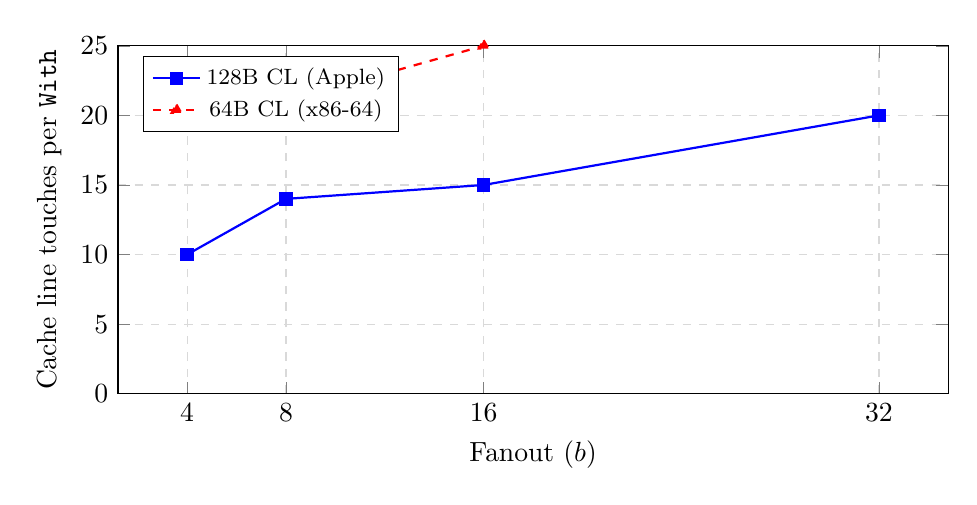
\begin{tikzpicture}
\begin{axis}[
    width=\columnwidth,
    height=6cm,
    xlabel={Fanout ($b$)},
    ylabel={Cache line touches per \texttt{With}},
    xtick={4,8,16,32},
    ytick={0,5,10,15,20,25},
    ymin=0, ymax=25,
    grid=major,
    grid style={dashed, gray!30},
    legend pos=north west,
    legend style={font=\footnotesize},
]
\addplot[mark=square*, blue, thick] coordinates {
    (4, 10) (8, 14) (16, 15) (32, 20)
};
\addlegendentry{128B CL (Apple)}
\addplot[mark=triangle*, red, thick, dashed] coordinates {
    (4, 20) (8, 21) (16, 25) (32, 36)
};
\addlegendentry{64B CL (x86-64)}
\end{axis}
\end{tikzpicture}
\caption{Estimated total cache line touches per \texttt{With} operation at
  $n = 10^6$, computed as depth $\times$ cache lines per branch copy.
  Fanout~4 minimizes 128-byte CL touches but maximizes allocation count.}
\label{fig:cacheline}
\end{figure}

At fanout~4, each branch fits in a single 128-byte Apple cache line,
explaining the $-19\%$ Set-With improvement at $n = 1024$ (where depth is
only $\sim$5).
However, at $n = 10^6$, the depth penalty ($\sim$10 levels $\times$ 1
allocation each) overwhelms the cache benefit, producing a $+17\%$
regression.

\subsection{Fanout Discussion}

No single fanout dominates across all benchmarks (\cref{tab:fanout-time}).
The underlying tradeoff is between \emph{depth} (which determines allocation
count per immutable operation) and \emph{node size} (which determines copy
cost and GC scanning cost per allocation):

\begin{itemize}[nosep]
  \item \textbf{Fanout~4}: Minimizes copy bandwidth but creates too many
        levels. Loses at scale ($+47\%$ SetBuilder at 1Mi).
  \item \textbf{Fanout~8}: 95\% occupancy means minimal waste. Moderate
        depth. Best overall balance.
  \item \textbf{Fanout~16}: Erratic --- a $+62\%$ regression on Set-With
        at 1ki contradicts neighbors, likely due to cache/alignment effects
        at the 272-byte branch size.
  \item \textbf{Fanout~32}: 31\% occupancy wastes 69\% of copy bandwidth.
        Catastrophic for merge ($+154\%$) despite helping sequential paths.
\end{itemize}

% ============================================================================
\section{Compact Arrays Analysis}
\label{sec:compact}

Traditional HAMTs use compact (popcount-indexed) arrays, storing only
populated children~\cite{bagwell2001,steindorfer2015}.
In Go, this requires a slice (\texttt{[]node[T]}), which adds a 24-byte
header (pointer + length + capacity) and a separate heap allocation for the
backing array.

Given the measured 95\% occupancy at fanout~8 (\cref{sec:occupancy}),
compact arrays would save an average of 0.37 empty slots per branch ---
approximately 6 bytes.
In exchange, every immutable \texttt{With} would require two heap
allocations per branch level (one for the branch struct, one for the slice
backing array) instead of one.

Since our profiling (\cref{sec:inline}) showed that halving allocations per
level from 2 to 1 improved Set-With by 12\%, \emph{doubling} them back to 2
would likely produce a comparable regression.
The negligible space savings do not justify this cost.

This conclusion is specific to our occupancy profile.
For HAMTs with lower occupancy (e.g., fanout~32 at 31\%), compact arrays
would save substantially more space, potentially justifying the extra
allocation.

% ============================================================================
\section{Discussion}
\label{sec:discussion}

\subsection{Allocation Count Dominates Allocation Size}

The central finding of this work is that in Go's runtime environment,
\emph{allocation count} is a stronger performance predictor than
\emph{allocation size} for HAMT operations:

\begin{enumerate}[nosep]
  \item Boxing elimination removed allocations entirely (not merely resized
        them): $-75\%$ allocs, $-25\%$ time on merge paths.
  \item Inline copies halved per-level allocations: $-12\%$ time on
        Set-With despite zero change in total bytes.
  \item Fanout~32 reduced allocation count by $\sim 40\%$ but increased
        per-allocation size by 3.7$\times$: net regression on merge paths
        due to GC scanning overhead.
\end{enumerate}

This aligns with Go's GC architecture, where cost scales with the number of
pointer-containing objects rather than total heap size~\cite{hudson2018}.

\subsection{Go-Specific Constraints}

Several results are non-transferable to other languages:

\begin{description}[nosep,leftmargin=1em]
  \item[Interface overhead.] Each \texttt{node[T]} slot occupies 16 bytes
    (vs.\ 8 bytes for a raw pointer in C/Rust or a compressed oop on the
    JVM). This doubles the effective node size and favors lower fanout than
    JVM or native implementations.
  \item[Escape analysis.] The pattern \texttt{ret := *b; return \&ret} always
    heap-allocates because Go's compiler cannot prove the result doesn't
    escape. Languages with value semantics (Rust) or aggressive inlining
    (C++) could potentially avoid this allocation entirely.
  \item[No monomorphization.] Go generics use dictionary dispatch, making
    per-type function caching necessary. In Rust or C++, monomorphization
    would eliminate this overhead at compile time.
\end{description}

\subsection{Implications for HAMT Design in GC'd Languages}

Our results suggest the following design principles for HAMTs in
garbage-collected languages:

\begin{enumerate}[nosep]
  \item \textbf{Measure occupancy before choosing compact vs.\ fixed arrays.}
        At $\geq 90\%$ occupancy, compact arrays add allocation overhead
        for negligible savings.
  \item \textbf{Choose fanout to maximize occupancy, not minimize depth.}
        The asymptotically optimal fanout (which minimizes $\log_b n$) may
        produce sparse nodes with high per-copy waste.
  \item \textbf{Minimize allocation count per operation.}
        In GC'd runtimes, one 144-byte allocation is cheaper than two
        72-byte allocations, even though total bytes are identical.
  \item \textbf{Pre-resolve type-dependent functions.}
        In languages with runtime generics dispatch, caching resolved
        functions on long-lived objects (builders, args structs) eliminates
        per-operation dispatch overhead.
\end{enumerate}

% ============================================================================
\section{Threats to Validity}
\label{sec:threats}

\textbf{Hardware specificity.}
All measurements were taken on a single architecture (Apple M4 Max) with
128-byte L1 cache lines.
Results may differ on x86-64 (64-byte cache lines) or architectures with
different memory latency characteristics.

\textbf{Workload representativeness.}
Our benchmarks use sequential integer keys with uniform hash distribution.
Workloads with clustered keys, high collision rates, or skewed access
patterns may shift the fanout tradeoff.

\textbf{Go version dependency.}
Go's garbage collector and escape analysis are actively developed.
Future versions may change the relative cost of allocations, potentially
altering some of our conclusions.

\textbf{Statistical rigor.}
While we used \texttt{benchstat} for significance testing, some benchmarks
used only 5 samples, which limits confidence intervals.

% ============================================================================
\section{Conclusion}
\label{sec:conclusion}

We presented a systematic optimization study of a Go HAMT implementation,
recovering from regressions of up to 56\% and achieving net improvements of
up to 46\% on key benchmarks.
The three implemented optimizations --- boxing elimination, concurrent map
bypass, and inline structural copying --- share a common theme: reducing
the number of heap allocations per operation.

Our exploration of branching factors (4, 8, 16, 32) revealed that the
existing 8-way fanout achieves 95\% slot occupancy, making it near-optimal
for Go's memory model.
This high occupancy also renders compact (variable-length) node arrays
counterproductive, since the space savings are negligible while the extra
allocation per node is costly.

The key insight is that HAMT optimization in garbage-collected languages
requires reasoning about the \emph{runtime cost model} (allocation count,
GC scanning, cache behavior) rather than purely about the \emph{data
structure} (depth, node size, asymptotic complexity).
A branching factor that is optimal on the JVM~\cite{steindorfer2015} or in
native code~\cite{bagwell2001} may be suboptimal in Go, and vice versa.

\section{Future Work}
\label{sec:future}

Beyond the remaining regressions, several promising directions remain
unexplored.

\subsection{\texttt{splitLeaf} Hot Path}

The primary source of the remaining Set-With regression ($+14$--$30\%$).
When two elements collide at a given hash prefix depth, \texttt{splitLeaf}
creates a full branch node plus two \texttt{leaf1} nodes --- three
allocations.
The eliminated \texttt{leaf2} stored two elements flat with zero branch
overhead.
Two approaches could address this:

\begin{description}[nosep,leftmargin=1em]
  \item[Specialized two-element node.] Restoring a \texttt{leaf2} type
    would eliminate branch creation for the common case of exactly two
    elements sharing a hash prefix, at the cost of $\sim$200 lines of
    additional type-switch cases.
  \item[Batch splitting.] When splitting a \texttt{leaf[T]} with $N$
    elements, partitioning all $N$ elements by their next hash chunk in a
    single pass would reduce intermediate allocations from $O(N)$ to
    $O(b)$, where $b$ is the fanout.
\end{description}

\subsection{IntSet/With Profiling}

The steepest remaining regression ($+62\%$) has not been profiled
independently.
It is unclear whether the cause is the same \texttt{splitLeaf} overhead or
something specific to the bitmap-compressed integer encoding
(\texttt{Map[I, cellMask]}).
The bitmap layer adds its own \texttt{With} operations on top of the
tree's, so the regression may compound differently than for plain
\texttt{Set[T]}.
Dedicated CPU profiling of this path would clarify the root cause and
identify whether a targeted fix is possible.

\subsection{Lazy \texttt{branch.count}}

The \texttt{branch.count} field is maintained eagerly on every
\texttt{With}/\texttt{Without} mutation, requiring arithmetic at each
branch level.
If \texttt{Count()} is called infrequently relative to mutations, computing
the count lazily --- either on demand by summing children, or via a
dirty-flag cache --- could eliminate per-mutation overhead.
Profiling is needed to determine whether count maintenance is actually
visible in hot paths.

\subsection{Leaf Slice Preallocation}

When \texttt{splitLeaf} distributes $N$ elements into child nodes, the
resulting \texttt{leaf} slices grow dynamically.
Preallocating at the expected partition size ($N / b$ or a small constant)
could reduce GC pressure from intermediate slice growth.
The impact is likely small given that leaf sizes are bounded at 8 elements,
but the cost of measurement is low.

\subsection{\texttt{pkg/rel} Generics Migration}

The relational algebra subpackage (\texttt{pkg/rel/}) --- providing Tuple,
Relation, Join, CartesianProduct, and Project operations --- currently does
not compile against the generics-based API\@.
It uses pre-generic types (\texttt{frozen.Map} without type parameters,
\texttt{frozen.StringMapBuilder}, etc.)\ and methods that no longer exist
(\texttt{.Equal}, \texttt{.Hash} on value types).
A migration pass is required to instantiate generic types, replace removed
helper constructors, and update value types to satisfy the
\texttt{Key[T]} constraint interface.

\subsection{Linter Upgrade}

The current linter configuration targets \texttt{golangci-lint} v1.60.1.
Newer versions may support additional linters, improved analysis passes,
and updated rule sets that could identify further code quality
improvements.

% ============================================================================
\begin{thebibliography}{99}

\bibitem{bagwell2001}
P.~Bagwell,
``Ideal hash trees,''
EPFL Technical Report, 2001.

\bibitem{steindorfer2015}
M.~J. Steindorfer and J.~J. Vinju,
``Optimizing hash-array mapped tries for fast and lean immutable JVM
collections,''
in \emph{Proc.\ ACM SIGPLAN Conf.\ Object-Oriented Programming, Systems,
Languages, and Applications (OOPSLA)}, pp.~783--800, 2015.

\bibitem{hickey2008}
R.~Hickey,
``The Clojure programming language,''
in \emph{Proc.\ Dynamic Languages Symposium (DLS)}, 2008.

\bibitem{odersky2004}
M.~Odersky, P.~Altherr, V.~Cremet, et al.,
``An overview of the Scala programming language,''
EPFL Technical Report IC/2004/64, 2004.

\bibitem{tibell2014}
J.~Tibell and E.~Kmett,
``\texttt{unordered-containers}: Efficient hashing-based container types,''
Haskell package, 2014.
\url{https://hackage.haskell.org/package/unordered-containers}

\bibitem{stucki2015}
N.~Stucki, T.~Rompf, V.~Ureche, and P.~Bagwell,
``RRB vector: A practical general purpose immutable sequence,''
in \emph{Proc.\ ACM SIGPLAN Int.\ Conf.\ Functional Programming (ICFP)},
pp.~342--354, 2015.

\bibitem{prokopec2012}
A.~Prokopec, N.~G. Bronson, P.~Bagwell, and M.~Odersky,
``Concurrent tries with efficient non-blocking snapshots,''
in \emph{Proc.\ ACM SIGPLAN Symp.\ Principles and Practice of Parallel
Programming (PPoPP)}, pp.~151--160, 2012.

\bibitem{driscoll1989}
J.~R. Driscoll, N.~Sarnak, D.~D. Sleator, and R.~E. Tarjan,
``Making data structures persistent,''
\emph{Journal of Computer and System Sciences}, vol.~38, no.~1,
pp.~86--124, 1989.

\bibitem{hudson2018}
R.~Hudson,
``Getting to Go: The journey of Go's garbage collector,''
GopherCon 2018.
\url{https://go.dev/blog/ismmkeynote}

\bibitem{go118}
The Go Authors,
``Type parameters proposal,''
2022.
\url{https://go.googlesource.com/proposal/+/refs/heads/master/design/43651-type-parameters.md}

\bibitem{benchstat}
The Go Authors,
``\texttt{benchstat}: Compute statistical summaries of benchmark results,''
\url{https://pkg.go.dev/golang.org/x/perf/cmd/benchstat}

\end{thebibliography}

\end{document}
